\section{Kyoto as a Multi-Agent System}

Here we detail the design decisions made regarding the modelling of the Kyoto Protocol \textsc{cpr} and considerations involved in mapping the Kyoto Protocol to a multi-agent system simulation. In order to properly explain the implementation of any one component of our Kyoto Protocol system, we must first elaborate on the larger structure of the project, giving a high level overview of the framework our agents are built upon.

\subsection{Time}

For the purpose of our simulation we refer to time in terms of sessions, years, and ticks. Presage2 is a discrete time simulation engine and ticks in our simulation map directly to Presage2's discrete units of time. Years last for a number of ticks defined at simulation time. Sessions are composed of multiple years, with a default of 10. In the real world Kyoto Protocol, the length of a session is mutable depending on the global economic and political climate. However, we felt it was a suitable abstraction from reality to use a consistent length for sessions throughout any individual simulation.

\subsection{Energy Output}

Energy output is an estimator of a participant's productivity. This is calculated in our simulation as the theoretical \CO emission were the country's industry entirely carbon based. The calculation of a country's energy output depends on many economic factors, which would be too complex to accurately calculate for our model. We use two factors to calculate this; the country's carbon output and the percentage of its industry dependent on fossil fuels. Hence, energy output is calculated as: 

%
% MATHSIFY THIS SHIT
%

\begin{center}
energy output = carbon output / fossil fuel \%
\end{center}

%
% MATHSIFY THIS SHIT
%

\subsection{Economy}

As with real world governments, our models of agent behaviors are necessarily constrained by the funds available to their respective administrations in their efforts to conserve the environment. \textsc{gdp} is a readily accessible and, for the complexity of our simulation, suitably accurate representation of countries' relative wealth. However, our simulation represents only the Kyoto Protocol in isolation, and an associated model of the global economy would be required to accurately gauge individual spending on the numerous national and international projects flexibly related to the Kyoto Protocol. To abstract away this complexity, each country is allocated a portion of its \textsc{gdp} every year as spendable income on projects relating to the Kyoto Protocol.

Manipulation of a country's \textsc{gdp} growth rate is the primary way we represent economic growth or recession. The formulae involved in modeling \textsc{gdp} growth depend primarily on a country's energy output, as defined above. This encourages investment in industry to promote economic growth, making maximisation of \textsc{gdp} growth a contrary but still achievable objective when adhering to Kyoto Protocol targets. These formulae also discourage drastic cutbacks in industry, which is intended to be an emergency measure for countries that are unable to meet their targets. This penalisation encourages long term thinking in the agent's behaviour, and rewards careful investment and management of targets alongside economic priorities.

\subsection{Monitoring and Sanctioning}
At the end of every year in our simulation, monitoring and sanctioning are performed to manage the emissions targets and detect fraudulent emissions reports. Each country is queried for its emissions reports by the monitoring service. The service then monitors a selection of countries, extracting their true carbon emissions, representing an abstraction of investigation by the \textsc{unfccc}. The monitoring service carries out sanctioning, imposing financial penalties on cheaters and harsher targets on countries who report emissions above their targets. Once sanctioning has been completed, the targetting service assigns new emissions targets to each country and the simulation proceeds as normal.

\begin{figure}[h!]
	\centering
	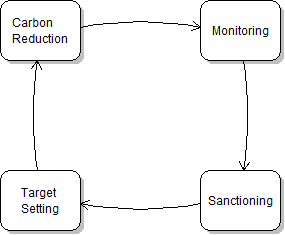
\includegraphics[width=\textwidth]{img/Kyoto_4_states.png}
	\caption{}
	\label{fig:kyoto_4_states}
\end{figure}

While we were eager to try and have our simulation model the Kyoto Protocol accurately, some changes needed to be made to discourage agents from abusing the game mechanics. For example, in a 10 year session, a participant could maximise their industry and \textsc{gdp} for the first 9 years and hence generate a large amount of funds. This could then be followed by a drastic reduction in industry to meet its target in the last year. This would create an excess of funds while the agent disregarded its emissions targets, giving it and unfair and unrealistic advantage.

\begin{description}
\item [Target Setting] \hfill \\ 
In the real world, targets are calculated per session for each participant. However, our model calculates the session target for each participant and then sets incremental, yearly targets which, if an individual country meets these targets, will ensure it meets its session target as well. This removes the potential abuse of the \textsc{gdp} functionality, since our simulated \textsc{gdp} is not externally sensitive to non-Kyoto Protocol events like \textsc{gdp} is in the real world.

\item [Reporting] \hfill \\ 
Our model follows the Kyoto Protocol and reporting is done yearly. Our reporting system is intentionally designed to allow countries to falsify their emissions reports, in the event that they, for any reason, wish to present incorrect emission data. One of the primary reasons for this would be not meeting emissions targets. At the risk of incurring financial penalties, it is possible for a country to avoid target sanctioning, which would have required an even more drastic reduction in the following year.

\item [Monitoring] \hfill \\ 
As per the \textsc{cpr} model, monitoring of participants should incur a cost. Every year all participants are `taxed' a certain percentage of their \textsc{gdp} in our model, which is used to cover the cost of monitoring participants. The Kyoto Protocol does not specifically call for a tax to cover its monitoring, although the \textsc{unfccc} is funded by its members, so our model represents a suitable abstraction from reality.

In the real world, monitoring is done every 5 years by a team of experts. We decided to monitor more frequently in order to discourage unrealistic participant behaviour. A number of random participants are checked yearly using the funds gained from the `monitor tax'. Repeat offenders, who have been found cheating before, have an increased probability of being monitored in the future.

\item [Sanctioning] \hfill \\ 
Sanctions are applied immediately when participants are found to have missed targets or have reported fraudulent emissions. The sanction for missing a target is a proportional increase in that participant's target in the following year, which is in line with the Kyoto Protocol regulations.

The sanction for fraudulent reporting in real life are rather `light weight', only suggesting a recalculation of the reported figures. In the real world, this kind of fraudulent activity would also result in political pressure from other Kyoto participants, but this would be difficult to model in our simulation. We wanted to look at the effect of a more `harsh' form of sanctioning, and thus we decided to impose financial sanctions for fraudulent reporting. This makes cheating, from an artificial intelligence perspective, a decision rather than a default. If the real world approach of simple target correction were employed then correctly reporting a failure to meet an emissions target is, from the isolated perspective represented in our simulation, never a sensible course of action. We wanted to avoid eliminating potential actions countries could take.
\end{description}

\subsection{Participants \& Actions}
Countries which form part of the Kyoto Protocol have been split into 4 groups:

\begin{itemize}
	\item{Annex I (Must reduce emissions -- e.g. \textsc{eu})}
	\item{Annex I (Must sustain emissions -- e.g. Russia)}
	\item{Non-Annex (Developing countries)}
	\item{Rogue States (Not part of Kyoto)}
\end{itemize}

While Annex I and Non-Annex countries have been implemented as per the Protocol specification, it was decided that we would remove the Annex II class (which is just a subset of Annex I), and allow all Annex I classes to invest in \textsc{cdm}.

Table X defined the actions which participants can use:

%TABLE
\begin{center}
ADD TABLE HERE
\end{center}
%TABLE

\subsubsection{Domestic Carbon Reduction Measures}

\begin{description}
\item [Carbon Absorption] \hfill \\ 
Carbon absorption is the process of building carbon sinks, projects which offset carbon emissions, for example planting large sections of forest. Our carbon absorption model allows for diminishing returns, so as more carbon absorption actions are taken, the return received for a given investment decreases. This models the changes in land price after extensive forestation, and the increased difficulty of building further carbon sinks as more projects are constructed. In theory, the cheaper, more efficient projects are prioritized, so once they have been completed, greater investment is required for further improvement.

Our model only allows for forestation on arable land; this differs from real life where trees can be planted on various types of land. This simplification allows us to use freely accessible country data. Another simplification is the immediate building/growing of trees; in real life, a participant would only get gradual carbon reduction gains from planting trees. However, there are mechanisms in place within the Kyoto Protocol to immediately reward member states for sustainable development projects which reduce long term emissions. Our carbon absorption system models an abstraction of these two factors combined. 

\item [Carbon Reduction] \hfill \\ 
Carbon reduction is the process of reducing carbon output of dirty industry. As in real life, our carbon reduction model allows for diminishing returns. Hence as more dirty industry is upgraded to clean one, the cost of further reduction increases. This maps to the ease of upgrading from coal power to existing, but cleaner natural gas technology, when compared to the investment required to pioneer nuclear fusion research.

Our model is only affected by the percentage of total dirty industry. In real life, there are various ways in which carbon reduction can be implemented, although the simplification used is suitable for the complexity of our model.

\item [Energy Usage] \hfill \\ 
As previously described, participants need to be able to have some influence over their \textsc{gdp} rate. In our model, energy output is a driving factor behind the \textsc{gdp} rate calculations, and so participants have the option of either growing or constricting their industry. This has the effect of changing the energy output and carbon output accordingly.

Investments in carbon industry will result in \textsc{gdp} growth, capped at sensible levels, but increases in carbon emissions. Countries who must reduce their overall emissions but wish to still maximize their economic growth must first invest in carbon industry and then in carbon reduction or absorption.
\end{description}

\subsubsection{Flexibility Mechanisms}

\begin{description}
\item [Emissions Trading] \hfill \\ 
In the real world, while being a viable carbon offsetting measure, carbon emission trading has proved less popular than domestic carbon reduction. Our model places more emphasis on emissions trading than in the real world, as we were interested in the simulation of an active commodities market.

It is understood that the world has several emission trading schemes and markets, the \textsc{eu ets} being one of the largest. While we did plan to incorporate the \textsc{eu ets} into our game, this was eventually scrapped as the time available did not warrant the extra complexity this would add to the simulation.

\item [Clean Development Mechanisms] \hfill \\
\textsc{cdm} is a significant action available to participants of the Kyoto Protocol, and similar to our interest in an active carbon market, we were keen to see the effects of an active market for clean investment. This mechanism is broadly unchanged from the real world specification, with the exception that we are not differentiating between \textsc{aau}s and \textsc{car}s.

\item [Joint Implementation] \hfill \\ 
The \textsc{ji} flexibility mechanism did not prove to be very popular in the real world, and with so few examples of this mechanism being carried out, it was left out of our simulation, and its inclusion would add unnecessary complexity.
\end{description}	
	
\subsection{Flowcharts}
Before moving to the coding phase of the project, some initial flow charts were drafted to help us visualise the different states and actions that would have to be implemented. The high level architecture of the simulation can be seen in Figure \ref{fig:kyoto_simulation_flowchart} with a more detailed composition of the country behaviour sub-process in Figure \ref{fig:country_behaviour_flowchart}:

\begin{figure}[h!]
	\centering
	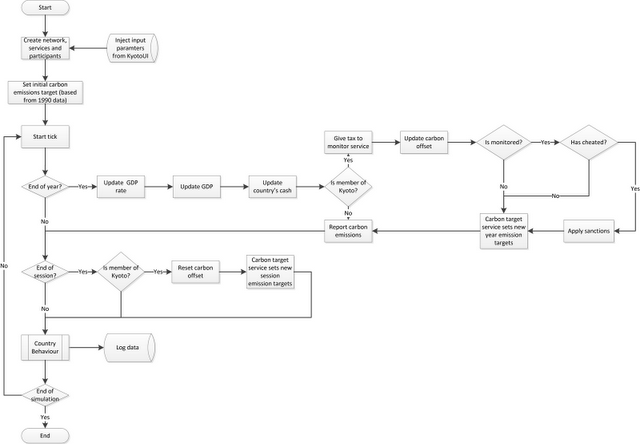
\includegraphics[width=0.8\textwidth]{img/kyoto_simulation_flowchart.png}
	\caption{Kyoto Simulation Flowchart}
	\label{fig:kyoto_simulation_flowchart}
\end{figure}

\begin{figure}[h!]
	\centering
	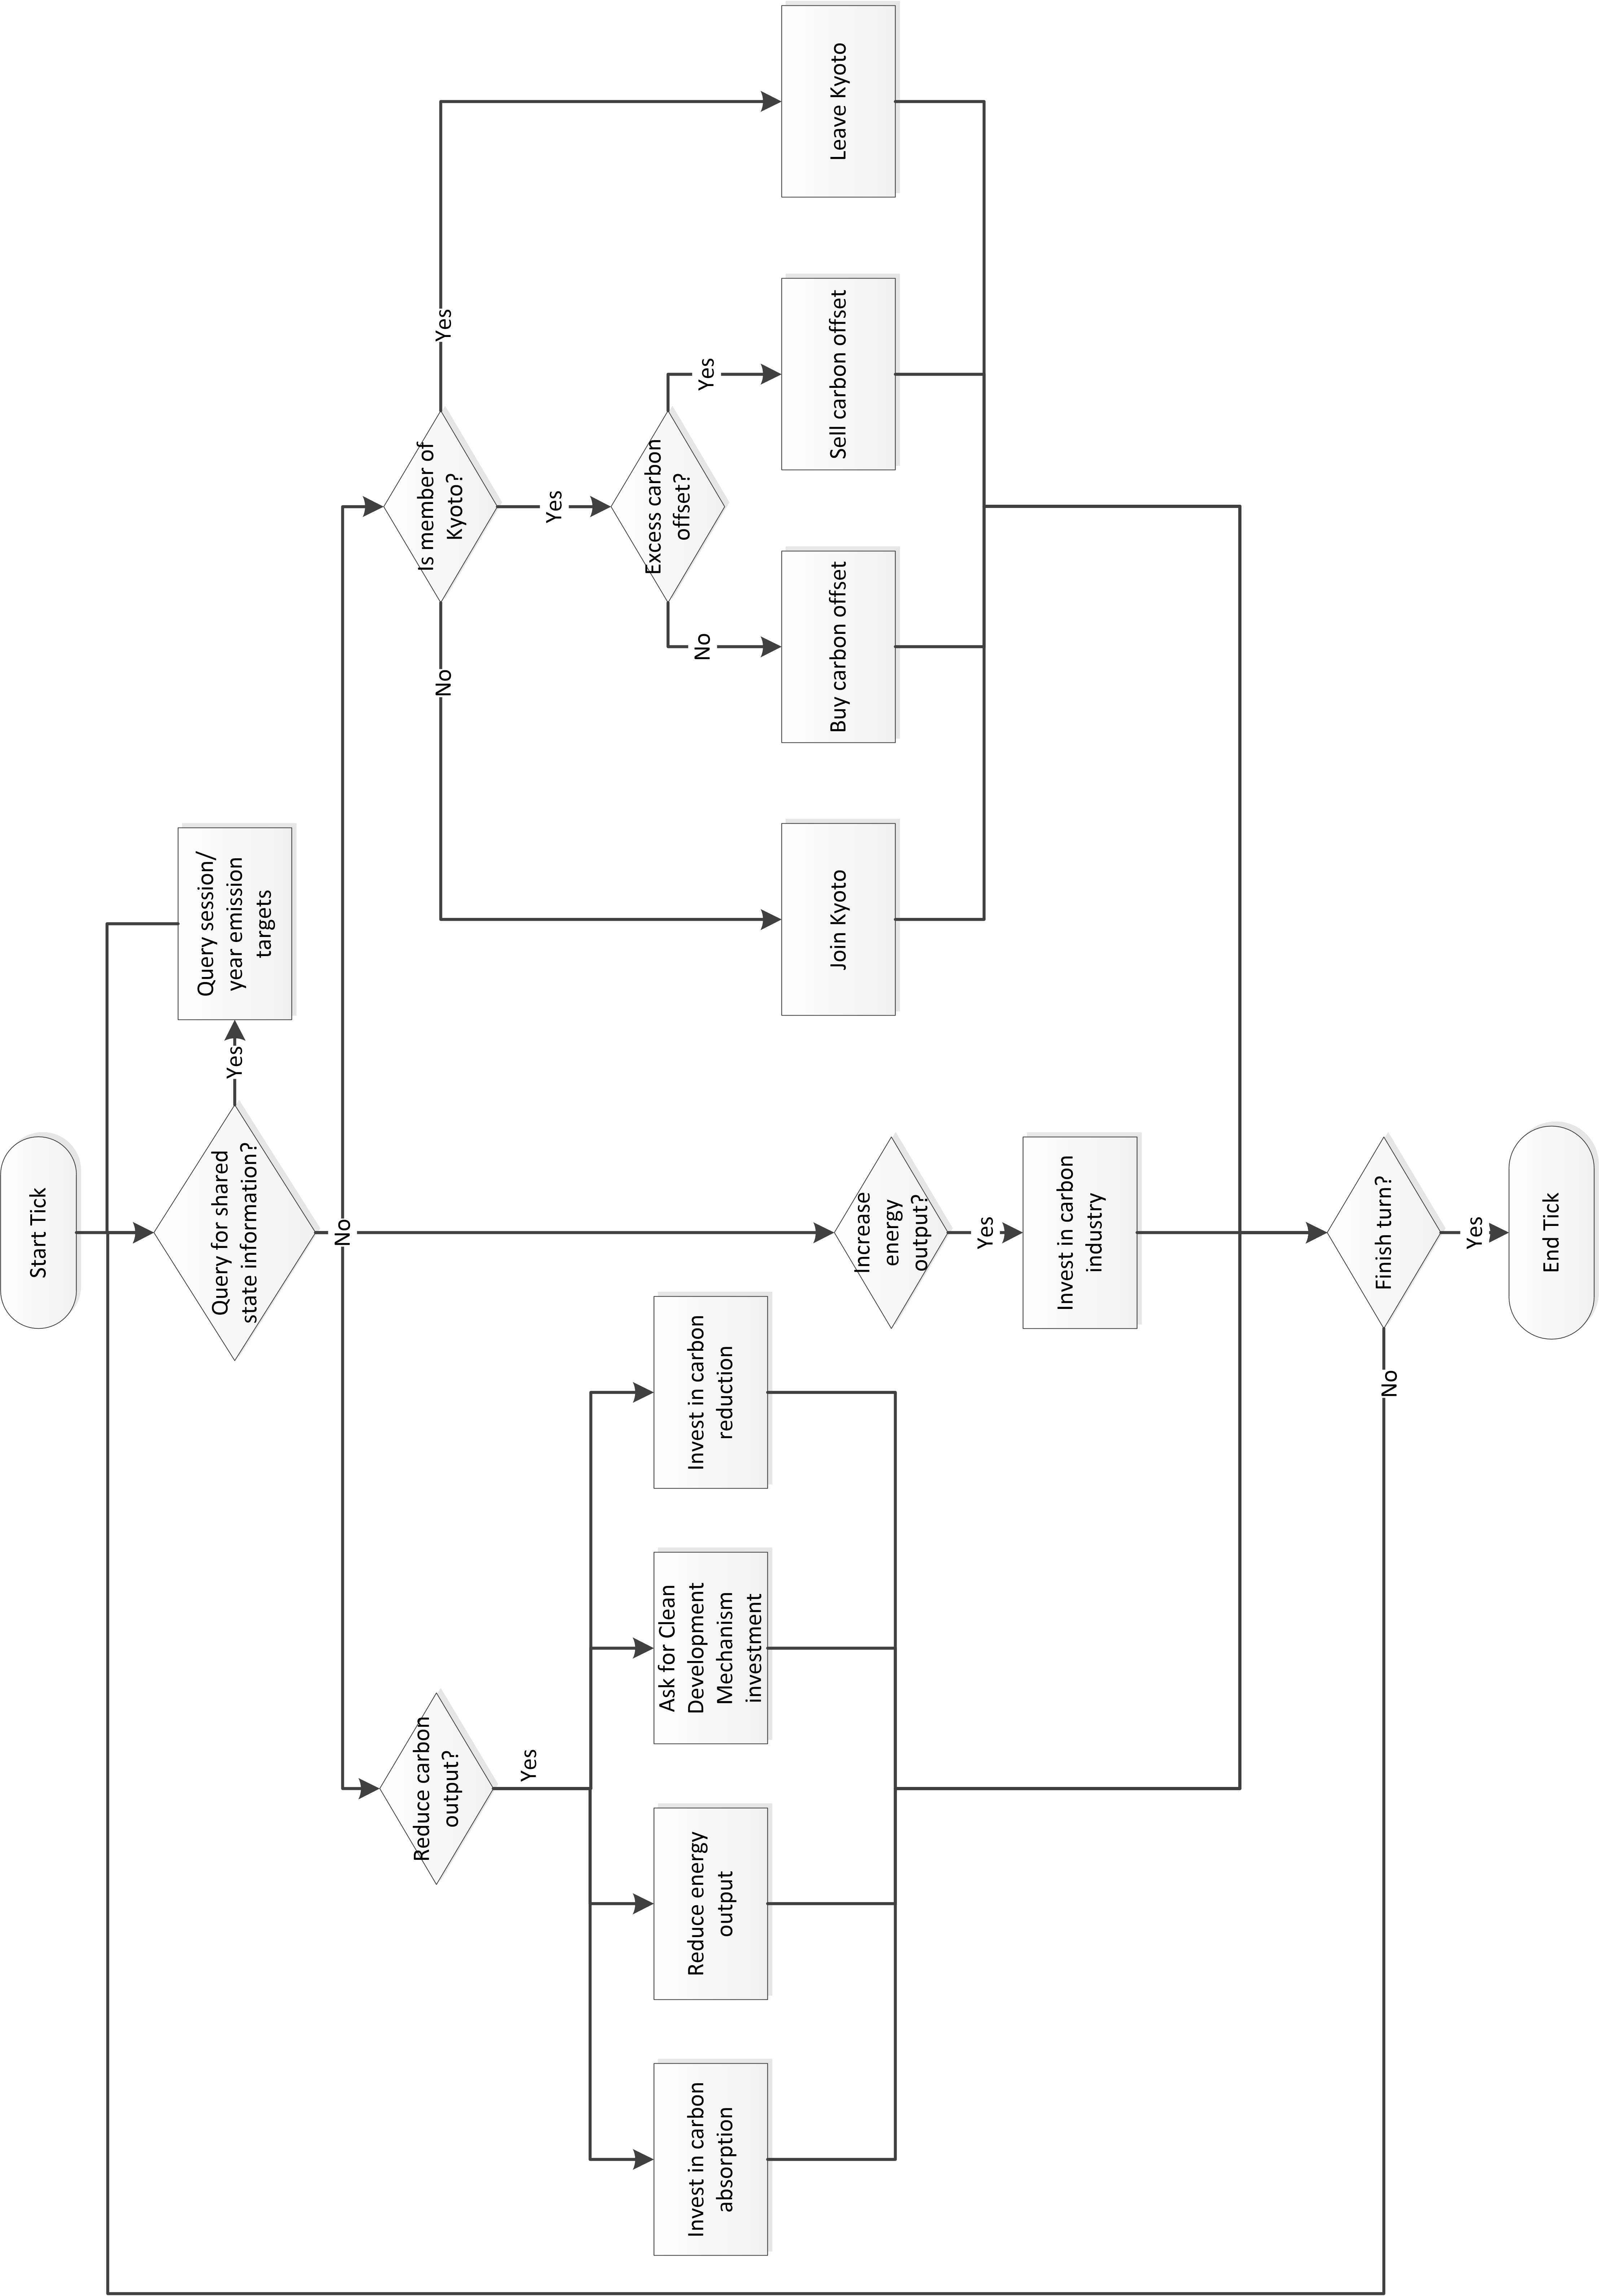
\includegraphics[width=0.8\textwidth]{img/country_behaviour_flowchart.png}
	\caption{Country Behaviour Flowchart}
	\label{fig:country_behaviour_flowchart}
\end{figure}
